
\section{ Implementation}
\begin{figure}[ht]
	\centering 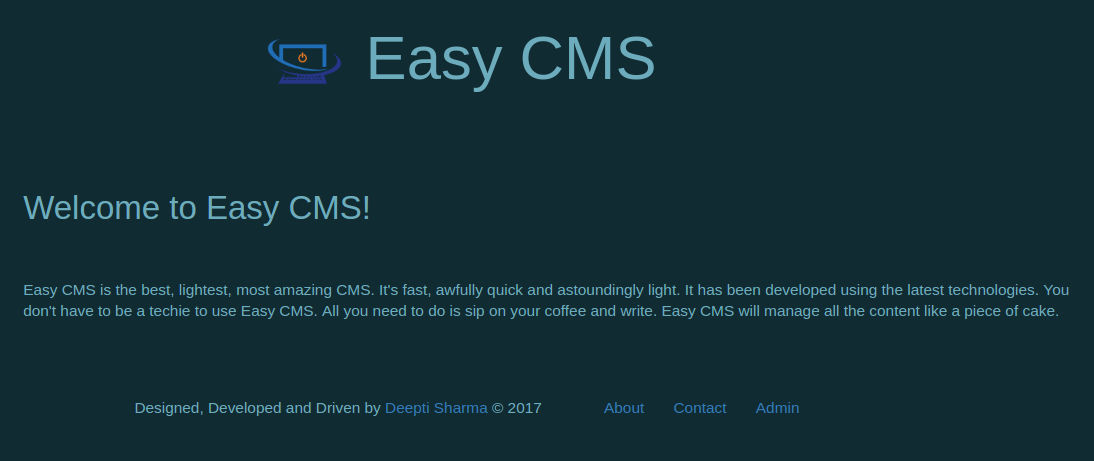
\includegraphics[scale=.45]{input/images/easy1.png}
	\caption{EasyCMS}
\end{figure}

 Easy CMS is the best, lightest, most amazing CMS. It's fast, awfully quick and astoundingly light. It has been developed using the latest technologies. You don't have to be a techie to use Easy CMS. All you need to do is sip on your coffee and write. Easy CMS will manage all the content like a piece of cake..\\
 

 \subsection{Login Panel}

 \begin{figure}[h!]
	\centering 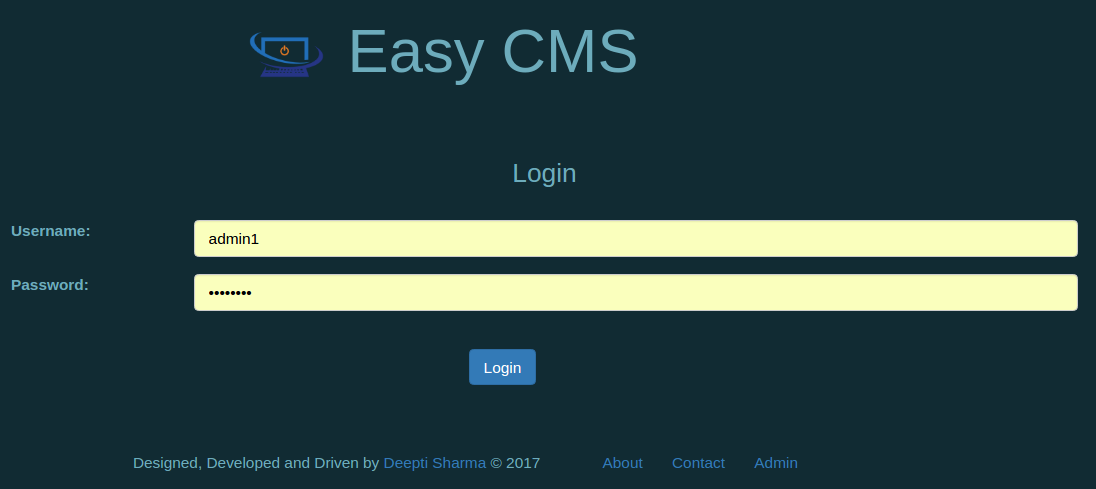
\includegraphics[scale=.45]{input/images/easy2.png}
	\caption{Login}
\end{figure}
This project is completely open source and the entire code is available 
to the user as and when required. There is Complete developer's 
Documentation as well as User manual alongwith it that helps using it a lot easier.\\
Moreover, anyone can use this service and need not have dependencies installed on their systems and can use this service remotely.\\\\

\subsection{Admin Panel}
\begin{figure}[h!]
	\centering 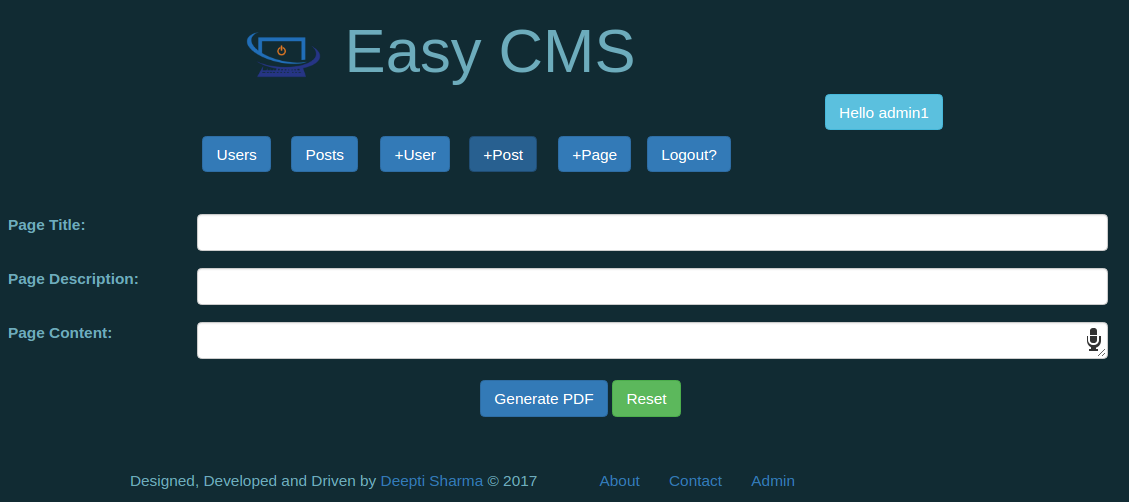
\includegraphics[scale=.45]{input/images/easy3.png}
	\caption{Admin Panel}
\end{figure}

\begin{figure}[h!]
	\centering 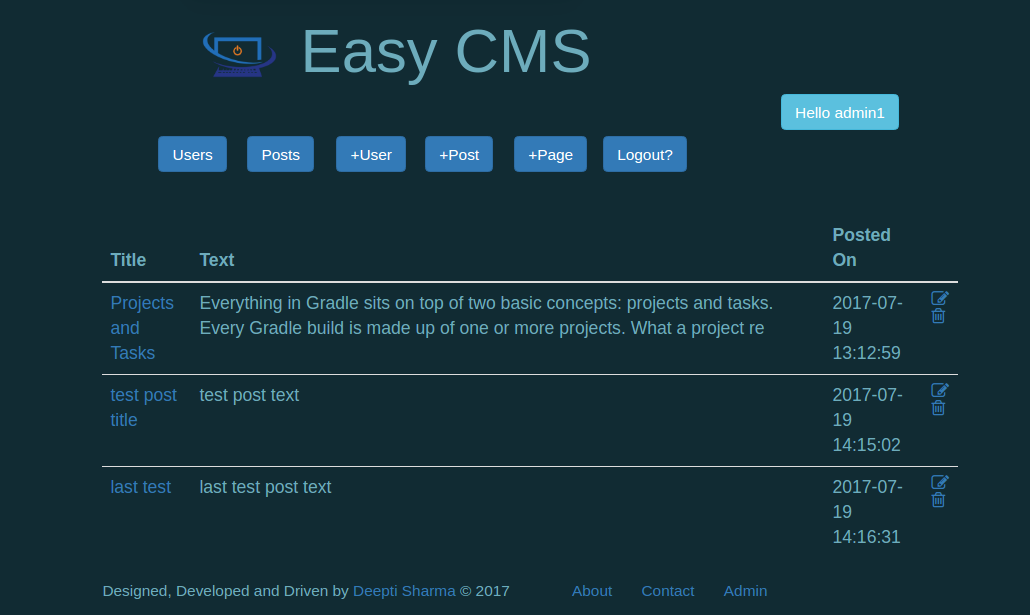
\includegraphics[scale=.49]{input/images/posts.png}
	\caption{Posts}
\end{figure}
Users can create different posts in this and are provided with a secure gateway to login. It provides many features like User creation and speech-recognision which makes it a little different.\\\\


\subsection{Users Control}
\begin{figure}[h!]
	\centering 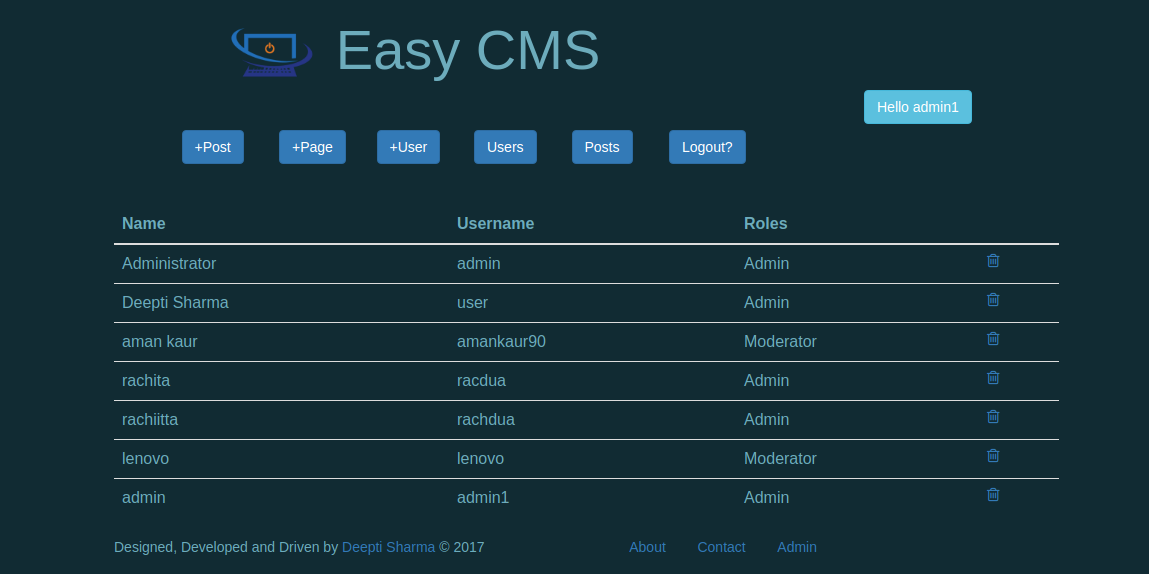
\includegraphics[scale=.44]{input/images/new.png}
	\caption{Admin Role}
\end{figure}

Using this feature, CMS can be used in a private firm who want to give access to their employees only.

\newpage
 \textbf{GNU/Linux systems:}
 
The working of Content Management System has been checked on various distributions of Linux such as several versions of Ubuntu including 12.04.5 and 14.04.5 (LTS). It was also checked on Fedora and Manjaro. Also a light weight operating system i.e Lubuntu.\\
 
 \textbf{Sources:}
 
Few sources which I considered while building this software are:
\begin{itemize}
\item Quora
\item Online Channels
\item Stack Overflow
\end{itemize}

 

 
  
